\section{DNA Thermodynamics}

 The field of DNA thermodynamics focuses on understanding how the structure of DNA varies
with temperature. Due to the nature of hydrogen bond interactions, that give rise to the
structure of dsDNA, the association and dissociation of the DNA duplex is possible. The
former is called DNA hybridisation shown in fig. ..., driven by a reduction in free
energy due to the bonding of complementary base-pairs. The latter is called DNA
melting, a process observed at high temperatures. This dissociation is
energetically driven, since the reduction in free energy due to base-pair hybridisation
is no longer a favourable trade-off with the reduction in configurational entropy in the
duplex structure.

During the discussion of the DNA nanopiston, we stated that thermodynamic transitions of
DNA are the driving force behind its operating cycle. The power stroke of the piston is
induced by a toehold mediated strand displacement reaction, while a hybridisation
reaction facilitates the recovery stroke.

Initiating a hybridisation reaction between two strands of ssDNA incurs a thermodynamic
penalty. This penalty originates in the decrease of configurational entropy, when the
strands start to form a duplex. This has a consequence that initial contacts in these
reactions often dissociate, due to the initial energy barrier that needs to be crossed
before the full hybridisation becomes energetically favourable. Even when an initial
contact
results in the stabilisation of a dsDNA duplex for select base-pairs, the configuration
often times is not conducive to full duplex formation. Especially in repetitive
sequences, the chance of a mismatched initial hybridisation is significant.

Another limiting factor to the rate constant of hybridisation reactions is that these
transitions are not characterised by a single state, but rather by an ensemble of
possible transition pathways. The number of pathways increase dramatically when the
strand sequences are repetitive, giving rise to hybridisation pathways facilitated by
Inchworm and pseudo-knot displacements[.].

The combination of the unstable initialisation of hybridisation reactions together
with its many transition pathways, complicates the analysis of the full reaction kinetics
observed in DNA hybridisation.


\begin{figure}[ht]
  \begin{centering}
  \adjustbox{minipage=1.3em,valign=t}{\subcaption{}\label{sfig:testa}}%
  \hspace{-0.3cm}
  \begin{subfigure}[t]{\dimexpr.2\linewidth-1.3em\relax}
  \centering
  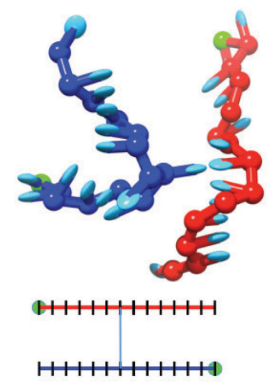
\includegraphics[width=1.06\linewidth,valign=t]{Figures/hybridDiag1.png}
  \end{subfigure}%
  \adjustbox{minipage=1.3em,valign=t}{\subcaption{}\label{sfig:testa}}%
  \hspace{-0.35cm}
  \begin{subfigure}[t]{\dimexpr.2\linewidth-1.3em\relax}
  \centering
  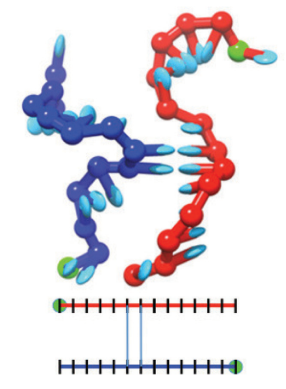
\includegraphics[width=1.09\linewidth,valign=t]{Figures/hybridDiag2.png}
  \end{subfigure}%
  \adjustbox{minipage=1.3em,valign=t}{\subcaption{}\label{sfig:testb}}%
  \hspace{-0.28cm}
  \begin{subfigure}[t]{\dimexpr.2\linewidth-1.3em\relax}
  \centering
  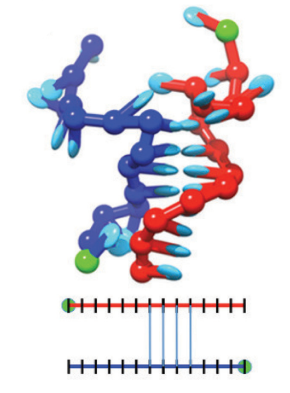
\includegraphics[width=1.1\linewidth,valign=t]{Figures/hybridDiag3.png}
  \end{subfigure}
  \adjustbox{minipage=1.3em,valign=t}{\subcaption{}\label{sfig:testa}}%
  \hspace{-0.21cm}
  \begin{subfigure}[t]{\dimexpr.2\linewidth-1.3em\relax}
  \centering
  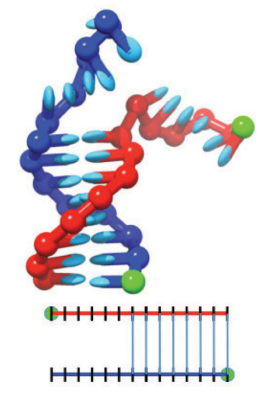
\includegraphics[width=.98\linewidth,valign=t]{Figures/hybridDiag4.png}
  \end{subfigure}%
  \adjustbox{minipage=1.3em,valign=t}{\subcaption{}\label{sfig:testa}}%
  \hspace{-0.38cm}
  \begin{subfigure}[t]{\dimexpr.2\linewidth-1.3em\relax}
  \centering
  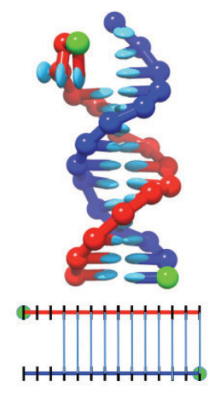
\includegraphics[width=.8\linewidth,valign=t]{Figures/hybridDiag5.png}
  \end{subfigure}
  % \adjustbox{minipage=1.3em,valign=t}{\subcaption{}\label{sfig:testb}}%
  % \hspace{-0.5cm}
  % \begin{subfigure}[t]{\dimexpr.2\linewidth-1.3em\relax}
  % \centering
  % 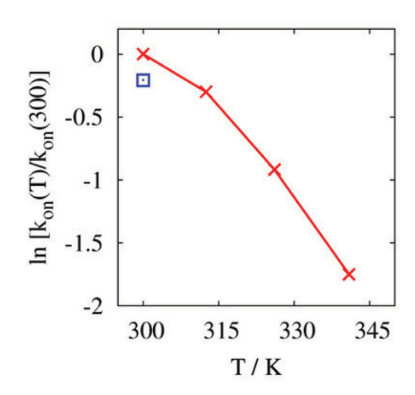
\includegraphics[width=1.5\linewidth,valign=t]{Figures/hybridDiag6.png}
  % \end{subfigure}
  \caption{This is a figure [.]}
  \label{fig:test}
  \end{centering}

\end{figure}

% ‘fraying’ to describe the disruption of base-pairs at the end of a duplex; if all base
% pairs fray, the duplex melts or dissociates.
%
% ‘zippering’ refers to when a new base-pair forms at the end of an existing duplex, shown
% in figure 3.2

The other important thermodynamic transition in the operating cycle of the nanopiston
is a toehold mediated strand displacement. Initially this reaction consists out of two
components. The first is an imperfect duplex structure, formed by a substrate strand and
an incumbent strand. The two strands are partially complementary by having either a
mismatch in their base-pair sequence or a surplus of base-pairs on the substrate strand.
The non-hybridised part of the substrate constitutes a flexible strand of ssDNA
that is referred to as the toehold.

The second component is called the invasive strand, and is fully complementary with the
substrate. It is energetically favourable for the invading
strand to disrupt the imperfect duplex structure and form a fully Watson–Crick
complementary dsDNA with the substrate strand. This displacement reaction results in an
overall reduction in the free energy of the system, since the strand displacement
increases the total number of hybridised base-pairs.

The process of strand displacement starts with the hybridisation of the toehold and the
invading strand. Once this initial hybridisation has occurred the invading strand can
start to contest hybridised base-pairs of the imperfect duplex. Disrupting the
base-pairing of the duplex is referred to as fraying, while the reverse process
where new base-pairs are formed is called zippering. During this process the invading
strand competes with the incumbent strand to form base-pairs with the substrate.

The reaction can be modelled using an one-dimensional energy landscape, called the
intuitive energy landscape (IEL) model[.], shown in figure ... . In the shape of the
energy landscape we recognise two distinct features. The first features is the initial
energy barrier, also seen in DNA hybridisation. This energy barrier again arises from a
reduction in configurational entropy, when the initial binding happens. The second
feature
is the plateau, representing the change in free energy when the strand
displacement takes place. This plateau gives rise to a relatively slow reaction, which
can be explained using a simple toy model. Considering a scenario, where the substrate
consists of $N+1$ nucleotide, with only one of these nucleotides constituting the
toehold. If we now assume that both the incumbent and invasive strand contest each others
hybridised base-pairs at the same rate, the displacement reaction can be modelled as a
random walk. The model is reduced to a famous problem in probability theory, called the
gamblers ruin. It can be shown that the reaction rate scales as $1/3N$[.], making the
Toehold displacement reaction increasingly difficult to study for large strands.

These two types of thermodynamic transitions, central in the operation cycle of the DNA
nanopiston, are relatively difficult to study due to their slow reaction rates and
initial energy barrier. Accurately analysing the reaction kinetics of these rare events,
requires the use of advanced sampling techniques.

\begin{figure}[ht]
\begin{center}
  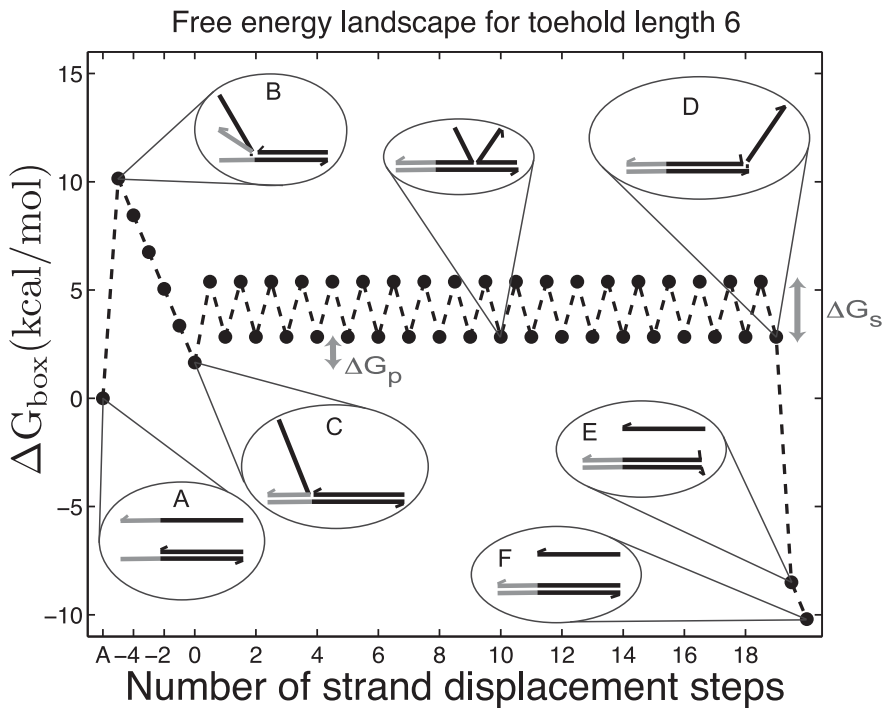
\includegraphics[width=0.6\textwidth]{Figures/ToeholdDiagram.png}
  \caption{write caption[.]}
\end{center}
\end{figure}


